\tikzset{>=latex} % for LaTeX arrow head

\colorlet{myblue}{blue!20}
\colorlet{mydarkblue}{blue!50!black}
\colorlet{myred}{black!50!red}

\tikzset{
  cube/.pic={
    \tikzset{every edge quotes/.append style={midway,auto},/cube/.cd,#1}
    \def\csize{2*\cubesize}
    \draw [every edge/.append style={pic actions,densely dashed,opacity=.5},pic actions]
    (0,0,0) coordinate (o)
            edge coordinate [pos=1] (g) ++(0,0,-\csize)
        --++(0,\csize,0) coordinate (a)
        --++(\csize,0,0) coordinate (b)
        --++(0,-\csize,0) coordinate (c) -- cycle
    (a) --++(0,0,-\csize) coordinate (d) edge (g)
        --++(\csize,0,0) coordinate (e) -- (b) -- cycle
    (c) -- (b) -- (e)
        --++(0,-\csize,0) coordinate (f) edge (g) -- cycle;
    \path [every edge/.append style={pic actions, |-|}];
  },
  z={(-0.334,-0.334)},
  /cube/.search also={/tikz},
  /cube/.cd,
  size/.store in=\cubesize, size=1,
}

\tikzset{
  gasparticle/.pic={
    \tikzset{/gasparticle/.cd,#1}
    \draw[->,green!60!black] (0,0) -- (\vec);
    \node[circle,fill,inner sep=.8,fill=black!80!blue] at (0,0,0) {};
  }
  /gasparticle/.search also={/tikz},
  /gasparticle/.cd,
  vec/.store in=\vec, vec={90:0.5},
}

% GAS in a box



% HOT BALLOON


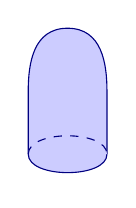
\begin{tikzpicture}[yscale=0.8]
  \draw[mydarkblue,fill=myblue]
    (-.5,0) -- (-.5,1) to[out=90,in=180] (0,2) to[out=0,in=90] (.5,1) -- (.5,0);
  \draw[dashed,mydarkblue,fill=myblue]
    (-.5,0) to[out=90,in=90] (.5,0);
  \draw[mydarkblue,fill=myblue]
    (-.5,0) to[out=-90,in=-90] (.5,0);
\end{tikzpicture}
